\subsection{Antena dla promieniowania THz, oparta na wzbudzeniu modu falowodowego}
Projektowana antena promieniowania THz powinna nie tylko zapewniać selektywność reakcji na promieniowanie E-M z wąskiego zakresu długości fali, co można uzyskać przy pomocy mechanizmów opisanych w paragrafie \ref{subart:rezo-grating}, ale również umożliwiać wzbudzenie detektora zlokalizowanego w małym obszarze przy pomocy promieniowania padającego na dowolną część anteny. Kompletny schemat układu anteny wraz z podkładem w którym umieszczony jest detektor promieniowania THz w postaci tranzystora polowego przedstawia rysunek \ref{fig:schem-podklad-falo}.
\begin{figure}
	\centering
	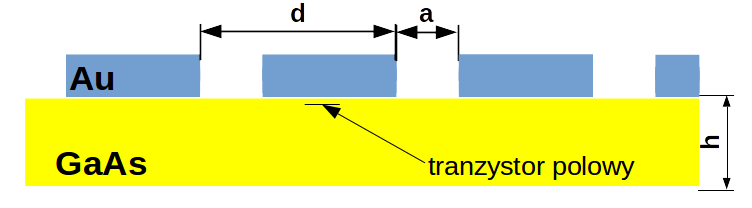
\includegraphics[width=\textwidth]{images/thz/schemat-podklad-falo.png}
	\caption{Schemat detektora promieniowania THz opartego na tranzystorze polowym}
	\label{fig:schem-podklad-falo}
\end{figure}

Rozkład pola na rysunku \ref{fig:consrcl525} nie zapewnia transportu promieniowania E-M w kierunku tranzystora polowego. W tym celu wykorzystany zostanie falowód tworzony przez podkład z $GaAs$. Siatka dyfrakcyjna tworząca antenę zostanie w tym przypadku wykorzystana w celu dopasowania pędu fali padającej do pędu modu falowodowego. W tym celu należy rozwiązać równanie dyspersji modów falowodowych\cite{petykiewicz1989podstawy}:
\begin{equation}
	\begin{gathered}
	\delta [ \kappa \textrm{cos}(\kappa h) + \gamma\textrm{sin}(\kappa h) ] - \kappa [ \kappa \textrm{sin}(\kappa h) - \gamma \textrm{cos}(\kappa h) = 0,\\
	\textrm{gdzie }\delta=\sqrt{\beta^2-\omega^2\mu_0},\textrm{ a }\kappa=\sqrt{\omega^2\mu_0\varepsilon_{\textrm{GaAs}}-\beta^2}.
	\end{gathered}
\end{equation}
Wszystkie wartości $\beta$ spełniające powyższą równość są dopuszczalnymi wartościamy składowej wektora falowego w kierunku propagacji, w ten sposób efektywne współczynniki załamania modów TM w falowodzie planarnym można obliczyć jako $n_{\textrm{eff}}=\frac{|k|}{\beta}$. Rozwiązanie powyższego równania możliwe jest jedynie na drodze graficznej lub numerycznej. W przypadku rozważanych podkładów z $GaAs$ $h=$400~$\mu m$, możliwe wartości efektywnego współczynnika załamania przedstawia wykres \ref{fig:gaas-effn}. Na podstawie tych wyników przygotowano wykres prezentujący okresy siatki $d$ potrzebne do wzbudzenia kolejnych modów falowodowych w zależności od długości fali dla której pracować ma antena, wyniki te prezenutje wykres \ref{fig:d-lusok}.

Bazując na pracach numerycznych na jednowymiarowych siatkach dyfrakcyjnych pozwalajachych na wzbudzenie modow falowodowych w podkladach z GaAs przeanalizowane zostalo dzialanie analogicznych falowodow zbudowanych z siatek koncentrycznych. 

Bazujac na analitycznym rozwiazaniu problemu wzbudzania modow falowodowych w podkladzie dielektrycznym (przy zalozeniu nieskonczonych wymiarow w kierunku propagacji wewnatrz falowodu) sporzadzono wykres przedstawiajacy zaleznosc okresu siatki pozwalajacej na wzbudzenie modu falowodowego od dlugosci fali w prozni promieniowania padajacego na uklad.

\begin{figure}
\begin{subfigure}{0.5\textwidth}
        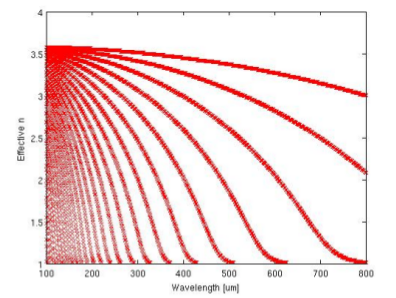
\includegraphics[width=\textwidth]{pomocnicze/thz/gaas-neffeps.png}
	\caption{Zależność $n_{\textrm{eff}}$ od długości fali}
	\label{fig:gaas-effn}
\end{subfigure}
\begin{subfigure}{0.5\textwidth}
        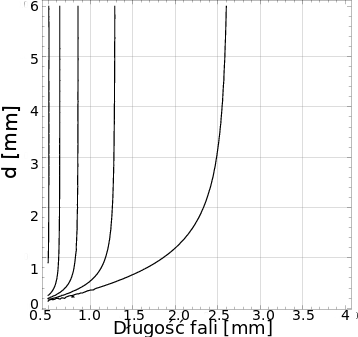
\includegraphics[width=\textwidth]{images/antenaThz/d_lambda.png}
	\caption{Wykres łączący okres siatki dyfrakcyjnej z długością fali dla której pracuje antena}
	\label{fig:d-lusok}
\end{subfigure}
\caption{Wyniki rozwiązania problemu falowodu planarnego o grubości $h=$400~$\mu$m z GaAs.}
\end{figure}

Wielosc galezi wynika z faktu, ze dla krotszych dlugosci fali rozpatrywany podklad ma charakter wielomodowy. Pojedyncze rozwiazanie powyzej dlugosci fali rownej 3mm, wskazuje nam poczatek zakresu jednomodowego.

\begin{figure}

\includegraphics{images/antenaThz/ro_consrc_radial_antena.png}
\end{figure}

Dla weryfikacji mozliwosci dzialania zaprojektowanych falowodow, przeprowadzono symulacje FDTD we wspolrzednych cylindryczncych. Symulacje potwierdzily mozliwosc wykorzystanie powyzszych siatek zarowno przy oswietleniu ukladu polaryzacja radialna jak  i liniowa. Ponizej przedstawiony rysunek opisuje sytuacje w ktorej struktura z GaAs o rozmiarach 10x10mm pokryta siatka dyfrakcyjna o okresie 538 um i otworach 250um (wspolczynnik wypelnienia ok. 0.53) zostala oswietlona promieniowaniem o dlugosci fali 2.52 mm. W przypadku prezentowanej symulacji siatka miala grubosc 10um, w kolejnych symulacjach potwierdzono jednak, ze grubosc siatki nie ma kluczowego zanczenia pod warunkiem zapewnienia nie przezroczystosci siatki. Efekt koncentracji pola przy zblizaniu sie do srodka struktury wynika ze zmniejszania sie elementu objetosciowego wraz ze zblizaniem do osi symetrii. 



